% !TeX program = xelatex
% !TeX root = main.tex

\documentclass[t,aspectratio=169,11pt]{beamer}

\usepackage{fontspec}
\defaultfontfeatures{Ligatures=TeX}
\IfFontExistsTF{Times New Roman}{
  \setmainfont{Times New Roman}
  \setsansfont{Times New Roman}
}{
  \setmainfont{TeX Gyre Termes}
  \setsansfont{TeX Gyre Termes}
}
\usefonttheme{serif}

\usepackage{amsmath,amssymb,mathtools,booktabs}
\usepackage{graphicx}
\usepackage{ragged2e}

% Cau hinh le cho HUST theme.
\def\slideContentLeftMargin{0.85cm}
\def\slideContentRightMargin{0.95cm}
\def\hustHeaderHeight{1.05cm}
\def\slideContentBotMargin{2.0cm}

% Template dang dung bo nen blue cua HUST.
\usepackage[blue,169]{beamerthemeHUST}
\graphicspath{{figures/}{images/}}

\renewcommand{\titlePageTitleX}{-0.45cm}
\renewcommand{\titlePageTitleY}{-0.35cm}
\renewcommand{\hustTitleAlign}{\alignLeft}
\renewcommand{\hustSubtitleAlign}{\alignLeft}
\renewcommand{\hustAuthorAlign}{\alignLeft}
\renewcommand{\hustInstAlign}{\alignLeft}

\newcommand{\trans}{^{\mathsf T}}
\newcommand{\inv}{^{-1}}
\newcommand{\vect}[1]{\boldsymbol{#1}}
\newcommand{\mat}[1]{\mathbf{#1}}

\newcommand{\sectionframe}[1]{%
  {%
    \setbeamertemplate{background}{%
      \includegraphics[width=\paperwidth,height=\paperheight]{\hustbg{section}}%
    }%
    \begin{frame}[plain,c]
      \centering
      \vfill
      \begin{minipage}{0.86\paperwidth}
        \centering
        {\Huge\bfseries\color{white}\thesection.\hspace{0.25em}#1\par}
      \end{minipage}
      \vfill
    \end{frame}%
  }%
  \useStyleHustFull%
  \useThinBar%
}

\newcommand{\sectionframeplain}[1]{%
  {%
    \setbeamertemplate{background}{%
      \includegraphics[width=\paperwidth,height=\paperheight]{\hustbg{section}}%
    }%
    \begin{frame}[plain,c]
      \centering
      \vfill
      \begin{minipage}{0.86\paperwidth}
        \centering
        {\Huge\bfseries\color{white}#1\par}
      \end{minipage}
      \vfill
    \end{frame}%
  }%
  \useStyleHustFull%
  \useThinBar%
}

\title[Suy luận về vectơ trung bình]{Suy luận về vectơ trung bình}
\subtitle{Chapter 5 - Applied Multivariate Statistical Analysis}
\author{Nhóm thuyết trình}
\institute{Đại học Bách khoa Hà Nội}
\date{\today}

\begin{document}

\hidePageNumber
\hustintropage{Chapter 5}
\husttitlepage

\begin{frame}{Thành viên nhóm}
  \vspace{0.15cm}
  \begin{columns}[T,onlytextwidth]
    \column{0.24\textwidth}
      \vspace{0.25cm}
      {\color{hustprimary}\fontsize{46}{50}\selectfont\bfseries 02\par}
      \vspace{0.1cm}
      {\Large\bfseries Nhóm thuyết trình\par}
      \vspace{0.25cm}
      {\color{hustprimary}\rule{0.82\linewidth}{1.2pt}\par}
      \vspace{0.25cm}
      {\color{hustprimary}\Large\bfseries 9\par}
      {\small thành viên\par}

    \column{0.36\textwidth}
      \small
      \renewcommand{\arraystretch}{1.18}
      \begin{tabular}{@{}l@{\hspace{0.28cm}}r@{}}
        \textbf{Họ và Tên} & \textbf{MSSV} \\
        \midrule
        Trần Lương Anh & 20237298 \\
        Trần Long Vũ & 20237409 \\
        Nguyễn Minh Đức & 20237313 \\
        Nguyễn Bá Đức Huy & 20237345 \\
        Hồ Xuân Bắc & 20237301 \\
      \end{tabular}

    \column{0.36\textwidth}
      \small
      \renewcommand{\arraystretch}{1.18}
      \begin{tabular}{@{}l@{\hspace{0.28cm}}r@{}}
        \textbf{Họ và Tên} & \textbf{MSSV} \\
        \midrule
        Nguyễn Xuân Cường & 20237307 \\
        Nguyễn Thị Thảo & 202419101 \\
        Vũ Công Hiệp & 20237328 \\
        Phạm Minh Hiếu & 20237331 \\
      \end{tabular}
  \end{columns}
\end{frame}

\begin{frame}{Mục lục}
  \vspace{0.05cm}
  \begingroup
  \normalsize
  \renewcommand{\arraystretch}{1.12}
  \setlength{\tabcolsep}{0pt}
  \begin{tabular}{@{}r@{\hspace{0.55em}}p{0.86\textwidth}@{}}
    {\color{hustprimary}\bfseries 1.} & \hyperlink{Navigation5}{Giới thiệu} \\[0.09cm]
    {\color{hustprimary}\bfseries 2.} & \hyperlink{Navigation9}{Tính hợp lý của \(\boldsymbol{\mu}_0\)} \\[0.09cm]
    {\color{hustprimary}\bfseries 3.} & \hyperlink{Navigation27}{Kiểm định Hotelling \(T^2\) và kiểm định tỷ số hợp lý} \\[0.09cm]
    {\color{hustprimary}\bfseries 4.} & \hyperlink{Navigation49}{Miền tin cậy và so sánh đồng thời} \\[0.09cm]
    {\color{hustprimary}\bfseries 5.} & \hyperlink{Navigation99}{Suy luận mẫu lớn về vectơ trung bình tổng thể} \\[0.09cm]
    {\color{hustprimary}\bfseries 6.} & \hyperlink{Navigation111}{Biểu đồ kiểm soát chất lượng đa biến} \\[0.14cm]
    & \hyperlink{exercises-start}{Bài tập và ví dụ tính toán}
  \end{tabular}
  \endgroup
\end{frame}

\resetPageCount
\showPageNumber
\useStyleHustFull
\useThinBar

% Pham vi goc: Muc 5.1 - Gioi thieu.
% File nay chi chia khuc noi dung, chua gan ten thanh vien phu trach.
\section{Giới thiệu}
\sectionframe{Giới thiệu}

\begin{frame}{Giới thiệu}
  \begin{block}{Phạm vi nội dung}
    Trình bày bối cảnh của chương: từ các khái niệm chương 1--4 chuyển sang suy luận thống kê cho vectơ trung bình tổng thể.
  \end{block}
  \begin{itemize}
    \item Mục tiêu của suy luận thống kê trong phân tích đa biến.
    \item Vì sao các biến tương quan cần được phân tích đồng thời.
    \item Vai trò của khoảng tin cậy đồng thời trong chương này.
  \end{itemize}
\end{frame}

% Pham vi goc: Muc 5.2 - Tinh hop ly cua mu_0.
% File nay chi chia khuc noi dung, chua gan ten thanh vien phu trach.
\section{Tính hợp lý của \texorpdfstring{\(\boldsymbol{\mu}_0\)}{mu0}}
\sectionframe{Tính hợp lý của \(\boldsymbol{\mu}_0\)}

\begin{frame}{Tính hợp lý của \texorpdfstring{\(\boldsymbol{\mu}_0\)}{mu0}}
  \begin{block}{Phạm vi nội dung}
    Từ kiểm định trung bình một biến, mở rộng sang kiểm định vectơ trung bình tổng thể bằng thống kê Hotelling \(T^2\).
  \end{block}
  \begin{itemize}
    \item Nhắc lại giả thuyết \(H_0: \boldsymbol{\mu}=\boldsymbol{\mu}_0\).
    \item Diễn giải khoảng cách thống kê quan sát.
    \item Liên hệ giữa \(T^2\) và phân phối \(F\).
  \end{itemize}
\end{frame}

% Pham vi goc: Muc 5.3 - Hotelling T^2 va kiem dinh ty so hop ly.
% File nay chi chia khuc noi dung, chua gan ten thanh vien phu trach.
\section{Hotelling \texorpdfstring{\(T^2\)}{T2} và kiểm định tỷ số hợp lý}
\sectionframe{Hotelling \(T^2\) và kiểm định tỷ số hợp lý}

\begin{frame}{Hotelling \texorpdfstring{\(T^2\)}{T2} và kiểm định tỷ số hợp lý}
  \begin{block}{Phạm vi nội dung}
    Trình bày công thức Hotelling \(T^2\), tiêu chuẩn bác bỏ \(H_0\), và cách nhìn từ kiểm định tỷ số hợp lý.
  \end{block}
  \begin{itemize}
    \item Ý nghĩa hình học của khoảng cách Mahalanobis.
    \item Điều kiện áp dụng trong mẫu từ phân phối chuẩn đa biến.
    \item Cách đọc kết luận kiểm định trên slide.
  \end{itemize}
\end{frame}

% Pham vi goc: Muc 5.4 - Mien tin cay va so sanh dong thoi.
% File nay chi chia khuc noi dung, chua gan ten thanh vien phu trach.
\section{Miền tin cậy và so sánh đồng thời}
\sectionframe{Miền tin cậy và so sánh đồng thời}

\begin{frame}{Miền tin cậy và so sánh đồng thời}
  \begin{block}{Phạm vi nội dung}
    Chuyển từ kiểm định một điểm \(\boldsymbol{\mu}_0\) sang tập các giá trị \(\boldsymbol{\mu}\) còn hợp lý với dữ liệu.
  \end{block}
  \begin{itemize}
    \item Miền tin cậy đồng thời cho vectơ trung bình.
    \item So sánh đồng thời các trung bình thành phần.
    \item Cách diễn giải miền ellipsoid hoặc khoảng tin cậy Bonferroni.
  \end{itemize}
\end{frame}
% =====================================================================
% PHẦN NỘI DUNG: NGUYỄN MINH ĐỨC
% =====================================================================

% Mục 5.4 - Phần 3: Phương pháp so sánh bội Bonferroni và phần kết
\begin{frame}{Động cơ: khi chỉ quan tâm các trung bình thành phần}
  \begin{itemize}
    \item Khoảng $T^2$ quá rộng nếu chỉ áp dụng cho riêng $p$ trung bình thành phần.
    \item Xét Hình 5.2: nếu $\mu_1$ nằm trong khoảng $T^2$ của nó và $\mu_2$ nằm trong khoảng $T^2$ của nó thì $(\mu_1,\mu_2)$ nằm trong hình chữ nhật tạo bởi hai khoảng này.
    \item Hình chữ nhật này \textbf{chứa elip tin cậy và còn hơn thế nữa}: xác suất phủ đồng thời $\mu_1,\mu_2$ lớn hơn $0{,}95$.
    \item Thông thường, ta chỉ quan tâm một \textbf{số nhỏ} $m$ phát biểu tin cậy $\Rightarrow$ có thể xây dựng khoảng đồng thời \textbf{ngắn hơn (chính xác hơn)} khoảng $T^2$.
    \item Cách làm này gọi là \textbf{phương pháp Bonferroni}, vì xuất phát từ một bất đẳng thức xác suất cùng tên.
  \end{itemize}
  \note{Câu hỏi có thể gặp: \emph{Vì sao $T^2$ quá rộng?} Vì khoảng $T^2$ đảm bảo cho mọi $\mathbf{a}$, còn ta chỉ cần $p$ trung bình. Hình chữ nhật tạo bởi các khoảng $T^2$ chứa elip tin cậy (elip có xác suất phủ đúng $0{,}95$) nên xác suất phủ của hình chữ nhật lớn hơn $0{,}95$, tức là ``dư'' độ tin cậy so với mức cần.}
\end{frame}
 
% ---------------------------------------------------------------------
\begin{frame}{Thiết lập bài toán}
  \begin{itemize}
    \item \textbf{Trước khi thu thập dữ liệu}, giả sử cần các phát biểu tin cậy về $m$ tổ hợp tuyến tính:
    \[
      \mathbf{a}_1'\boldsymbol{\mu},\; \mathbf{a}_2'\boldsymbol{\mu},\; \ldots,\; \mathbf{a}_m'\boldsymbol{\mu},
      \qquad \mathbf{a}'\boldsymbol{\mu} = a_1\mu_1 + a_2\mu_2 + \cdots + a_p\mu_p
    \]
    \item Gọi $C_i$ là phát biểu tin cậy về giá trị của $\mathbf{a}_i'\boldsymbol{\mu}$, với
    \[
      P[C_i \text{ đúng}] = 1-\alpha_i, \qquad i = 1,2,\ldots,m
    \]
    \item Mục tiêu: kiểm soát xác suất để \textbf{tất cả} $C_i$ cùng đúng.
  \end{itemize}
  \note{Câu hỏi có thể gặp: \emph{Vì sao phải chọn phát biểu trước khi thu thập dữ liệu?} Sách đặt giả thiết ``prior to the collection of data'' khi xây dựng phương pháp. Ngược lại, các khoảng $T^2$ ``lý tưởng cho dò quét dữ liệu'' vì hệ số tin cậy $1-\alpha$ không đổi với mọi cách chọn $\mathbf{a}$ (sách trang 226).}
\end{frame}
 
% ---------------------------------------------------------------------
\begin{frame}{Bất đẳng thức Bonferroni }
  \small
  \setlength{\abovedisplayskip}{2pt}
  \setlength{\belowdisplayskip}{2pt}
  \begin{align*}
    P[\text{tất cả } C_i \text{ đúng}] &= 1 - P[\text{ít nhất một } C_i \text{ sai}] \\
    &\ge 1 - \sum_{i=1}^m P(C_i \text{ sai}) = 1 - \sum_{i=1}^m \bigl(1 - P(C_i \text{ đúng})\bigr) \\
    &= 1 - (\alpha_1 + \alpha_2 + \cdots + \alpha_m) \tag{5-28}
  \end{align*}
  \footnotesize
  \begin{itemize}
    \item Cho phép kiểm soát \textbf{tỷ lệ sai số tổng thể} $\alpha_1+\cdots+\alpha_m$, \textbf{bất kể cấu trúc tương quan} đằng sau các phát biểu.
    \item Có thể kiểm soát tỷ lệ sai số cho một nhóm phát biểu quan trọng, và cân bằng bằng một lựa chọn khác cho các phát biểu ít quan trọng hơn.
  \end{itemize}
  \note{Câu hỏi có thể gặp: \emph{Bước dấu $\ge$ từ đâu?} Biến cố ``ít nhất một $C_i$ sai'' là hợp của các biến cố ``$C_i$ sai'', và xác suất của một hợp không vượt quá tổng các xác suất, nên $P[\text{ít nhất một sai}] \le \sum P(C_i \text{ sai})$; trừ hai vế từ $1$ ta được dấu $\ge$. Vì chỉ dùng tổng xác suất nên không cần biết các $C_i$ độc lập hay tương quan. Bước tiếp theo dùng $P(C_i \text{ sai}) = 1 - P(C_i \text{ đúng}) = \alpha_i$.}
\end{frame}
 
% ---------------------------------------------------------------------
\begin{frame}{Khoảng Bonferroni cho các trung bình thành phần}
  \begin{itemize}
    \item Không có thông tin về tầm quan trọng tương đối của các thành phần $\mu_i$ $\Rightarrow$ xét các khoảng $t$ riêng lẻ với $\alpha_i = \alpha/m$:
    \[
      \bar{x}_i \pm t_{n-1}\!\left(\frac{\alpha_i}{2}\right)\sqrt{\frac{s_{ii}}{n}}, \quad i=1,\ldots,m
    \]
    \item Vì $P\!\left[\bar{X}_i \pm t_{n-1}\!\left(\frac{\alpha}{2m}\right)\sqrt{\frac{S_{ii}}{n}} \text{ chứa } \mu_i\right] = 1-\frac{\alpha}{m}$, từ (5-28):
    \[
      P\!\left[\bar{X}_i \pm t_{n-1}\!\left(\tfrac{\alpha}{2m}\right)\sqrt{\tfrac{S_{ii}}{n}} \text{ chứa } \mu_i,\ \forall i\right]
      \ge 1 - \underbrace{\left(\tfrac{\alpha}{m}+\tfrac{\alpha}{m}+\cdots+\tfrac{\alpha}{m}\right)}_{m \text{ số hạng}} = 1-\alpha
    \]
  \end{itemize}
  \note{Câu hỏi có thể gặp: \emph{Vì sao là $t_{n-1}(\alpha/2m)$?} Khoảng $t$ hai phía có mức ý nghĩa $\alpha_i=\alpha/m$ dùng điểm phần trăm trên $100(\alpha_i/2)$ của phân phối $t$ với $n-1$ bậc tự do, tức $t_{n-1}\!\left(\frac{\alpha}{2m}\right)$ (cách định nghĩa $t_{n-1}(\alpha/2)$ ở trang 224). \emph{Vì sao chọn $\alpha_i=\alpha/m$?} Vì không biết thành phần nào quan trọng hơn, và $m$ số hạng $\alpha/m$ cộng lại đúng bằng $\alpha$.}
\end{frame}
 
% ---------------------------------------------------------------------
\begin{frame}{Khoảng Bonferroni và so sánh với khoảng $T^2$}
  Với mức tin cậy tổng thể $\ge 1-\alpha$, ta đưa ra $m=p$ phát biểu:
  \begin{equation*}
    \bar{x}_i - t_{n-1}\!\left(\frac{\alpha}{2p}\right)\sqrt{\frac{s_{ii}}{n}} \;\le\; \mu_i \;\le\; \bar{x}_i + t_{n-1}\!\left(\frac{\alpha}{2p}\right)\sqrt{\frac{s_{ii}}{n}}, \quad i=1,\dots,p \tag{5-29}
  \end{equation*}
  \begin{block}{So sánh (5-29) với (5-24)}
    Giá trị $t_{n-1}\!\left(\dfrac{\alpha}{2p}\right)$ thay cho $\sqrt{\dfrac{(n-1)\,p}{n-p}F_{p,n-p}(\alpha)}$; ngoài điểm thay thế này, các khoảng có \textbf{cùng cấu trúc}.
  \end{block}
  \note{Câu hỏi có thể gặp: \emph{Khác biệt duy nhất giữa hai phương pháp?} Chỉ ở hệ số nhân của $\sqrt{s_{ii}/n}$: $T^2$ dùng $\sqrt{p(n-1)F_{p,n-p}(\alpha)/(n-p)}$, Bonferroni dùng $t_{n-1}(\alpha/2p)$. Hai hệ số này được so sánh bằng số ở Bảng 5.4 (slide sau).}
\end{frame}
 
% ---------------------------------------------------------------------
\begin{frame}{Ví dụ 5.6: Khoảng Bonferroni 95\% (dữ liệu bức xạ lò vi sóng)}
  Dữ liệu ở Ví dụ 5.3 và 5.4: $n=42$, $p=2$, $\alpha_i = 0{,}05/2$, $i=1,2$.
  \[
    t_{41}\!\left(\frac{0{,}05}{2(2)}\right) = t_{41}(0{,}0125) = 2{,}327
  \]
  \begin{exampleblock}{Kết quả (hệ số $\sqrt{s_{ii}/n}$ lấy từ Ví dụ 5.3)}
    \begin{align*}
      \bar{x}_1 \pm t_{41}(0{,}0125)\sqrt{\tfrac{s_{11}}{n}} &= 0{,}564 \pm 2{,}327\sqrt{\tfrac{0{,}0144}{42}} \quad\text{hay}\quad 0{,}521 \le \mu_1 \le 0{,}607 \\[1ex]
      \bar{x}_2 \pm t_{41}(0{,}0125)\sqrt{\tfrac{s_{22}}{n}} &= 0{,}603 \pm 2{,}327\sqrt{\tfrac{0{,}0146}{42}} \quad\text{hay}\quad 0{,}560 \le \mu_2 \le 0{,}646
    \end{align*}
  \end{exampleblock}
  So với các khoảng $T^2$ ở Ví dụ 5.4: $(0{,}516;\,0{,}612)$ và $(0{,}555;\,0{,}651)$.
  \note{Câu hỏi có thể gặp: \emph{Giá trị $2{,}327$ từ đâu?} $m=p=2$ nên $\alpha/2m = 0{,}05/4 = 0{,}0125$; tra $t$ với $n-1=41$ bậc tự do ta được $t_{41}(0{,}0125)=2{,}327$ (theo sách). Các số $\bar{x}_1=0{,}564$, $\bar{x}_2=0{,}603$, $s_{11}=0{,}0144$, $s_{22}=0{,}0146$ lấy từ Ví dụ 5.3.}
\end{frame}
 
% ---------------------------------------------------------------------
\begin{frame}{Hình 5.4: Khoảng Bonferroni và khoảng $T^2$}
  \begin{columns}[T]
    \begin{column}{0.52\textwidth}
      \centering
      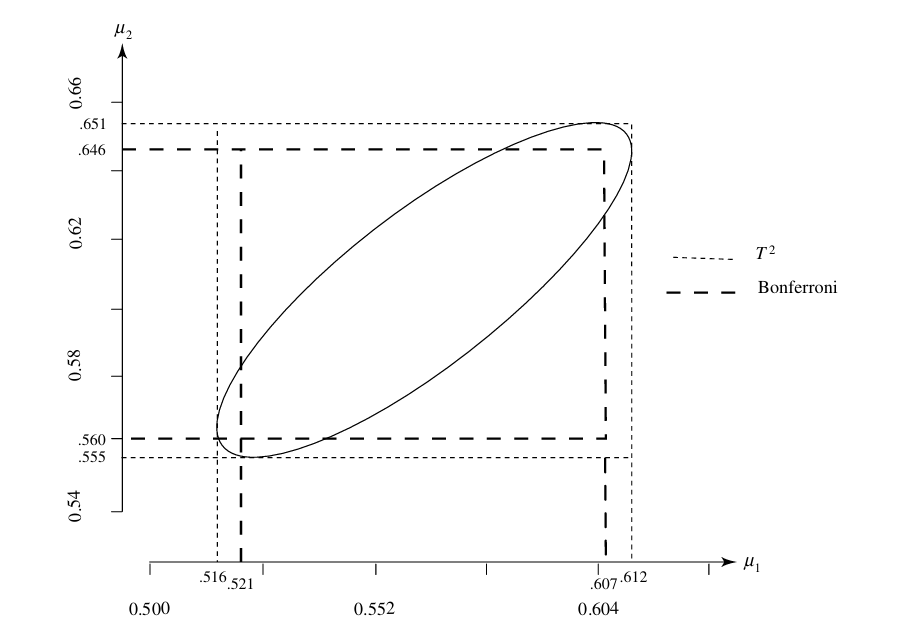
\includegraphics[width=\textwidth]{figures/figure_5_4.png}
    \end{column}
    \begin{column}{0.48\textwidth}
      \small
      \begin{itemize}
        \item Với mỗi trung bình thành phần, khoảng Bonferroni nằm \textbf{trong} khoảng $T^2$.
        \item Do đó hình chữ nhật tạo bởi hai khoảng Bonferroni nằm trong hình chữ nhật tạo bởi hai khoảng $T^2$.
        \item Nếu chỉ quan tâm các trung bình thành phần: Bonferroni cho ước lượng \textbf{chính xác hơn}.
        \item Miền tin cậy 95\% đối với $\boldsymbol{\mu}$ cho các giá trị hợp lý của cặp $(\mu_1,\mu_2)$ khi \textbf{tính đến tương quan} giữa các biến đo.
      \end{itemize}
    \end{column}
  \end{columns}
  \note{Chú ý: chú thích trong hình, đường chấm là khoảng $T^2$ (.516--.612; .555--.651), đường đứt nét là khoảng Bonferroni (.521--.607; .560--.646).}
\end{frame}
 
% ---------------------------------------------------------------------
\begin{frame}{So sánh độ dài: Bonferroni và $T^2$}
  \small
  \setlength{\abovedisplayskip}{2pt}
  \setlength{\belowdisplayskip}{2pt}
  Hai loại khoảng đều có dạng $\mathbf{a}'\bar{\mathbf{X}} \pm (\text{giá trị tới hạn})\sqrt{\mathbf{a}'\mathbf{S}\mathbf{a}/n}$. Khi $\alpha_i=\alpha/m$:
  \begin{equation*}
    \frac{\text{Độ dài khoảng Bonferroni}}{\text{Độ dài khoảng } T^2}
    = \frac{t_{n-1}(\alpha/2m)}{\sqrt{\dfrac{p(n-1)}{n-p}F_{p,n-p}(\alpha)}} \tag{5-30}
  \end{equation*}
  \vspace{-0.2cm}
  \begin{columns}[T]
    \begin{column}{0.46\textwidth}
      \footnotesize
      \begin{itemize}
        \item Tỷ số \textbf{không phụ thuộc} $\bar{\mathbf{X}}$ và $\mathbf{S}$.
        \item Với số nhỏ $m$ hàm $\mathbf{a}'\boldsymbol{\mu}$ chỉ định trước, khoảng Bonferroni luôn ngắn hơn; Bảng 5.4 cho thấy ngắn hơn bao nhiêu khi $m=p$.
      \end{itemize}
    \end{column}
    \begin{column}{0.52\textwidth}
      \centering
      {\scriptsize \textbf{Bảng 5.4} (Độ dài Bonferroni)/(Độ dài $T^2$), $1-\alpha=0{,}95$, $\alpha_i=0{,}05/m$\par}
      \vspace{2pt}
      \scriptsize
      \begin{tabular}{c|ccc}
        \toprule
        & \multicolumn{3}{c}{$m=p$} \\
        $n$ & 2 & 4 & 10 \\
        \midrule
        15       & 0,88 & 0,69 & 0,29 \\
        25       & 0,90 & 0,75 & 0,48 \\
        50       & 0,91 & 0,78 & 0,58 \\
        100      & 0,91 & 0,80 & 0,62 \\
        $\infty$ & 0,91 & 0,81 & 0,66 \\
        \bottomrule
      \end{tabular}
    \end{column}
  \end{columns}
  \note{Câu hỏi có thể gặp: \emph{Vì sao tỷ số không phụ thuộc $\bar{\mathbf{X}}$ và $\mathbf{S}$?} Hai loại khoảng có cùng dạng $\mathbf{a}'\bar{\mathbf{X}} \pm (\text{tới hạn})\sqrt{\mathbf{a}'\mathbf{S}\mathbf{a}/n}$, nên khi lập tỷ số độ dài, phần $\sqrt{\mathbf{a}'\mathbf{S}\mathbf{a}/n}$ triệt tiêu, chỉ còn tỷ số hai giá trị tới hạn. \emph{Đọc bảng thế nào?} Số $0{,}69$ ở $n=15$, $p=4$ nghĩa là khoảng Bonferroni chỉ dài bằng $69\%$ khoảng $T^2$.}
\end{frame}
 
% ---------------------------------------------------------------------
\begin{frame}{Khi nào dùng Bonferroni?}
  \begin{columns}[T]
    \begin{column}{0.48\textwidth}
      \begin{block}{Ưu điểm}
        \small
        \begin{itemize}
          \item Kiểm soát tỷ lệ sai số tổng thể $\alpha_1+\cdots+\alpha_m$, \textbf{bất kể cấu trúc tương quan}.
          \item Linh hoạt chia $\alpha_i$: nhóm phát biểu quan trọng dùng $\alpha_i$ khác với nhóm ít quan trọng.
          \item Với $m$ nhỏ, khoảng \textbf{ngắn hơn (chính xác hơn)} khoảng $T^2$ (Bảng 5.4).
          \item Dễ áp dụng, chỉ cần giá trị $t$.
        \end{itemize}
      \end{block}
    \end{column}
    \begin{column}{0.48\textwidth}
      \begin{block}{Phạm vi áp dụng}
        \small
        \begin{itemize}
          \item Chú ý đến một \textbf{số nhỏ} $m$ phát biểu tin cậy.
          \item Các phát biểu được \textbf{chỉ định trước khi thu thập dữ liệu}.
          \item Nếu muốn chọn $\mathbf{a}$ sau khi xem dữ liệu (dò quét dữ liệu), khoảng $T^2$ là lý tưởng vì $1-\alpha$ không đổi với mọi $\mathbf{a}$.
          \item Cho khoảng từng thành phần; để xét cặp $(\mu_i,\mu_k)$ có tính đến tương quan thì dùng elip tin cậy.
        \end{itemize}
      \end{block}
    \end{column}
  \end{columns}
  \note{Mọi ý trên đều có trong sách: ưu điểm ở trang 232 (bất đẳng thức 5-28 và hai nhận xét sau nó) và trang 234 (Bảng 5.4); phạm vi áp dụng ở trang 232 (``small number'', ``prior to the collection of data''), trang 226 (dò quét dữ liệu, elip 5-26) và trang 234 (miền tin cậy tính đến tương quan).}
\end{frame}
 
% ---------------------------------------------------------------------
\begin{frame}{Kết luận }
  \begin{itemize}
    \item Phương pháp Bonferroni cho khoảng \textbf{ngắn hơn} khi $m=p$ (Bảng 5.4).
    \item Vì \textbf{dễ áp dụng} và cho các khoảng tin cậy \textbf{tương đối ngắn} cần thiết cho suy diễn thống kê, ta thường áp dụng các \textbf{khoảng $t$ đồng thời dựa trên phương pháp Bonferroni}.
    \item Nếu cần các giá trị hợp lý cho cặp $(\mu_1,\mu_2)$ có tính đến tương quan giữa các biến, dùng \textbf{miền tin cậy} (elip) cho $\boldsymbol{\mu}$.
  \end{itemize}
  \note{Hai ý đầu là câu kết của mục 5.4 (trang 234). Ý thứ ba lấy từ cuối Ví dụ 5.6 (trang 233--234).}
\end{frame}
% Pham vi goc: Muc 5.5 - Suy luan mau lon.
% File nay chi chia khuc noi dung, chua gan ten thanh vien phu trach.
\section{Suy luận mẫu lớn về vectơ trung bình tổng thể}
\sectionframe{Suy luận mẫu lớn về vectơ trung bình tổng thể}

\begin{frame}{Suy luận mẫu lớn về vectơ trung bình tổng thể}
  \begin{block}{Phạm vi nội dung}
    Trình bày cách xấp xỉ mẫu lớn khi giả định chuẩn đa biến không còn là trọng tâm chính.
  \end{block}
  \begin{itemize}
    \item Vai trò của định lý giới hạn trung tâm đa biến.
    \item Dạng thống kê kiểm định và miền tin cậy khi \(n\) lớn.
    \item Điểm cần nhấn mạnh khi so sánh với trường hợp chuẩn đa biến.
  \end{itemize}
\end{frame}

% Pham vi goc: Muc 5.6 - Bieu do kiem soat chat luong da bien.
% File nay chi chia khuc noi dung, chua gan ten thanh vien phu trach.
\section{Biểu đồ kiểm soát chất lượng đa biến}
\sectionframe{Biểu đồ kiểm soát chất lượng đa biến}

\begin{frame}{Biểu đồ kiểm soát chất lượng đa biến}
  \begin{block}{Phạm vi nội dung}
    Kết nối Hotelling \(T^2\) với bài toán giám sát quá trình khi nhiều đặc trưng chất lượng được theo dõi đồng thời.
  \end{block}
  \begin{itemize}
    \item Ý tưởng phát hiện quan sát bất thường bằng \(T^2\).
    \item Cách xác định giới hạn kiểm soát.
    \item Diễn giải hình và bảng số liệu nếu đưa vào slide.
  \end{itemize}
\end{frame}

% Pham vi: Bai tap va vi du tinh toan.
% File nay chi chia khuc noi dung, chua gan ten thanh vien phu trach.
\section{Bài tập và ví dụ tính toán}
\sectionframe{Bài tập và ví dụ tính toán}

% Cac slide Bai 5.1--5.3 cua cac thanh vien khac co the dat truoc moc nay.
% BEGIN: Bai 5.4--5.5

\begin{frame}{Bài tập và ví dụ tính toán}
  \small
  {\large\textbf{Bài 5.4: đề bài trong sách}\par}
  \vspace{0.15cm}
  \begin{block}{Đề bài}
    Sử dụng dữ liệu mồ hôi trong Bảng 5.1 (xem Ví dụ 5.2).
    \begin{enumerate}
      \item[(a)] Xác định các trục của ellipsoid tin cậy \(90\%\) cho vectơ trung bình \(\vect{\mu}\) và độ dài của các trục này.
      \item[(b)] Vẽ biểu đồ Q--Q lần lượt cho các quan sát về tốc độ tiết mồ hôi, hàm lượng natri và hàm lượng kali. Vẽ ba biểu đồ phân tán khả dĩ cho từng cặp quan sát. Giả thiết phân phối chuẩn đa biến có hợp lý trong trường hợp này không? Hãy nhận xét.
    \end{enumerate}
  \end{block}
\end{frame}

\begin{frame}{Bài tập và ví dụ tính toán}
  \small
  {\large\textbf{Bài 5.4: dữ kiện dùng trong lời giải}\par}
  \vspace{0.1cm}
  \begin{columns}[T,onlytextwidth]
    \column{0.52\textwidth}
    \begin{block}{Dữ liệu từ Ví dụ 5.2}
      Với \(n=20,\ p=3\),
      \[
        \bar{\vect{x}}=
        \begin{bmatrix}
          4{,}640\\
          45{,}400\\
          9{,}965
        \end{bmatrix}
      \]
      \[
        \mat{S}=
        \begin{bmatrix}
          2{,}879 & 10{,}010 & -1{,}810\\
          10{,}010 & 199{,}788 & -5{,}640\\
          -1{,}810 & -5{,}640 & 3{,}628
        \end{bmatrix}.
      \]
    \end{block}

    \column{0.45\textwidth}
    \begin{block}{Ký hiệu}
      \begin{itemize}
        \item \(X_1\): tốc độ tiết mồ hôi.
        \item \(X_2\): hàm lượng natri.
        \item \(X_3\): hàm lượng kali.
        \item Câu (a) dùng trị riêng và vectơ riêng của \(\mat{S}\).
        \item Câu (b) kiểm tra trực quan qua Q--Q plot và scatter plot.
      \end{itemize}
    \end{block}
  \end{columns}
\end{frame}

\begin{frame}{Bài tập và ví dụ tính toán}
  \small
  {\large\textbf{Bài 5.4(a): trị riêng và hướng trục}\par}
  \vspace{0.1cm}
  Trục của ellipsoid đi theo các vectơ riêng chuẩn hóa của \(\mat{S}\). Trị riêng là nghiệm của
  \[
    |\mat{S}-\lambda\mat{I}|=0
    \quad\Longrightarrow\quad
    \lambda^3-206{,}295\lambda^2+1175{,}180\lambda-1181{,}529=0.
  \]

  \begin{block}{Cách chọn vectơ riêng}
    Với mỗi \(\lambda_i\), giải hệ thuần nhất
    \((\mat{S}-\lambda_i\mat{I})\vect{v}_i=\vect{0}\).
    Vectơ riêng chỉ xác định đến hằng số nhân khác \(0\), nên có thể đặt một thành phần thuận tiện bằng \(1\), rồi chuẩn hóa
    \(\vect{e}_i=\vect{v}_i/\|\vect{v}_i\|\).
  \end{block}

  \vspace{-0.1cm}
  \begin{center}
    \scriptsize
    \begin{tabular}{@{}c c c@{}}
      \toprule
      \(\lambda_i\) & \(\vect{v}_i\trans\) có thể chọn & \(\vect{e}_i\trans\) sau chuẩn hóa \\
      \midrule
      \(200{,}462\) & \([\,0{,}0509,\ 1,\ -0{,}0291\,]\) &
      \([\,0{,}051,\ 0{,}998,\ -0{,}029\,]\) \\
      \(4{,}533\) & \([\,1,\ -0{,}0924,\ -1{,}4245\,]\) &
      \([\,0{,}574,\ -0{,}053,\ -0{,}817\,]\) \\
      \(1{,}300\) & \([\,1,\ -0{,}0304,\ 0{,}7039\,]\) &
      \([\,0{,}817,\ -0{,}025,\ 0{,}575\,]\) \\
      \bottomrule
    \end{tabular}
  \end{center}
\end{frame}

\begin{frame}{Bài tập và ví dụ tính toán}
  \footnotesize
  {\large\textbf{Bài 5.4(a): độ dài các trục ellipsoid}\par}
  \vspace{-0.02cm}
  Ellipsoid tin cậy \(90\%\) có các nửa trục
  \[
    \pm\sqrt{\lambda_i}
    \sqrt{\frac{p(n-1)}{n(n-p)}F_{p,n-p}(\alpha)}\,\vect{e}_i,
    \qquad i=1,2,3.
  \]
  Với \(p=3,\ n=20,\ \alpha=0{,}10\) và \(F_{3,17}(0{,}10)\approx2{,}44\),
  \[
    \sqrt{\frac{3(19)}{20(17)}F_{3,17}(0{,}10)}
    \approx 0{,}640.
  \]

  \begin{center}
    \scriptsize
    \begin{tabular}{@{}c c c c@{}}
      \toprule
      Trục & \(\lambda_i\) & Nửa trục & Độ dài đầy đủ \\
      \midrule
      \(1\) & \(200{,}462\) & \(9{,}055\,\vect{e}_1\) & \(18{,}111\) \\
      \(2\) & \(4{,}533\)   & \(1{,}362\,\vect{e}_2\) & \(2{,}723\) \\
      \(3\) & \(1{,}300\)   & \(0{,}729\,\vect{e}_3\) & \(1{,}459\) \\
      \bottomrule
    \end{tabular}
  \end{center}
\end{frame}

\begin{frame}{Bài tập và ví dụ tính toán}
  \small
  {\large\textbf{Bài 5.4(b): cách dựng Q--Q plot}\par}
  \vspace{0.1cm}
  Theo Mục 4.6, trang 178--179, Q--Q plot so sánh phân vị mẫu với phân vị lý thuyết của phân phối chuẩn.
  Với mỗi biến \(X_k\), thực hiện:
  \begin{enumerate}
    \item Sắp xếp mẫu: \(x_{(1)k}\le x_{(2)k}\le \cdots \le x_{(20)k}\).
    \item Gán vị trí xác suất cho quan sát thứ \(j\): \(p_j=(j-\frac{1}{2})/n=(j-\frac{1}{2})/20\).
    \item Tính phân vị chuẩn lý thuyết: \(q_j=\Phi^{-1}(p_j)\).
  \end{enumerate}
  Các điểm được vẽ là \((q_j,\ x_{(j)k})\). Trục hoành là phân vị chuẩn lý thuyết, trục tung là dữ liệu đã sắp xếp.

  \vspace{0.15cm}
  {\footnotesize\textit{Chú thích:} Chuẩn đa biến là giả thiết về cả vectơ \(X=(X_1,X_2,X_3)^T\). Q--Q plot kiểm tra từng biến biên, còn scatter plot giúp nhìn quan hệ theo từng cặp biến.\par}
\end{frame}

\begin{frame}{Bài tập và ví dụ tính toán}
  \small
  \vspace{-0.2cm}
  \begin{center}
    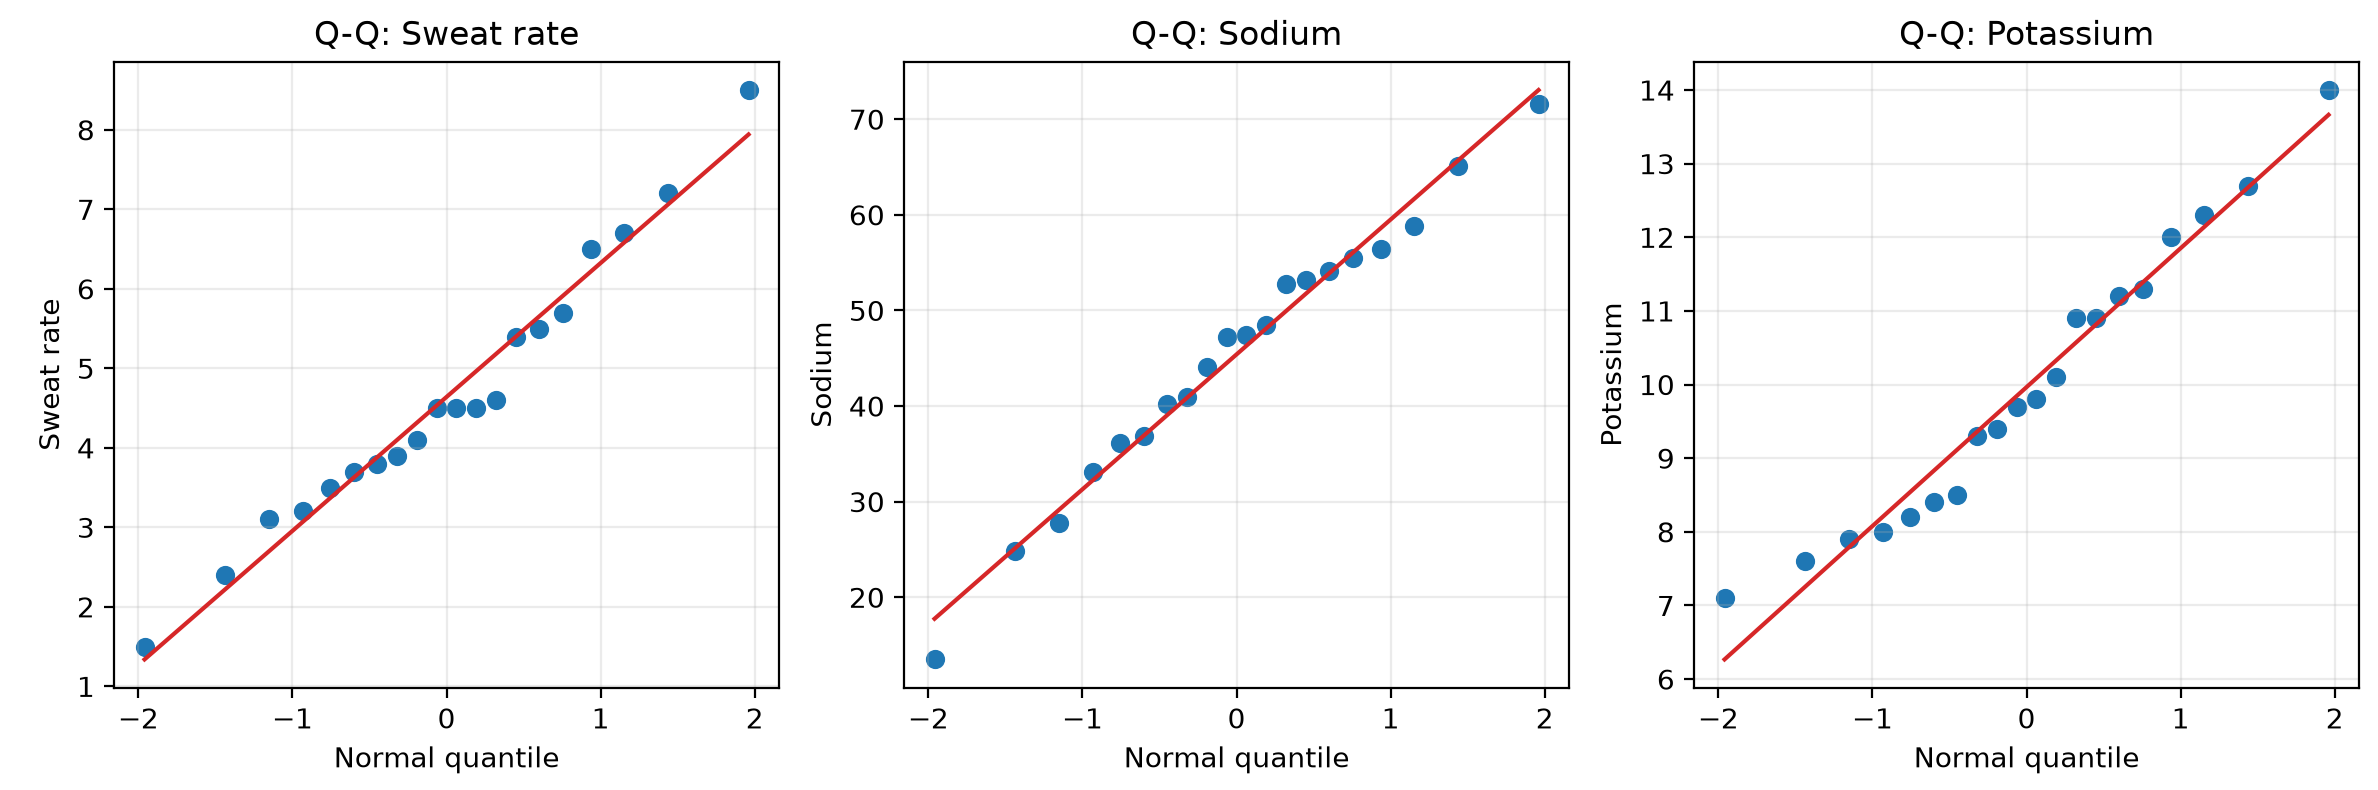
\includegraphics[width=0.96\textwidth,height=0.52\textheight,keepaspectratio]{exercise_5_4_qq.png}
  \end{center}
  \vspace{-0.15cm}
  \begin{block}{Nhận xét}
    Các điểm của ba Q--Q plot nhìn chung bám sát đường thẳng tham chiếu.
    Không thấy độ cong mạnh hoặc điểm lệch quá xa ở hai đầu phân phối.
  \end{block}
\end{frame}

\begin{frame}{Bài tập và ví dụ tính toán}
  \small
  \vspace{-0.2cm}
  \begin{center}
    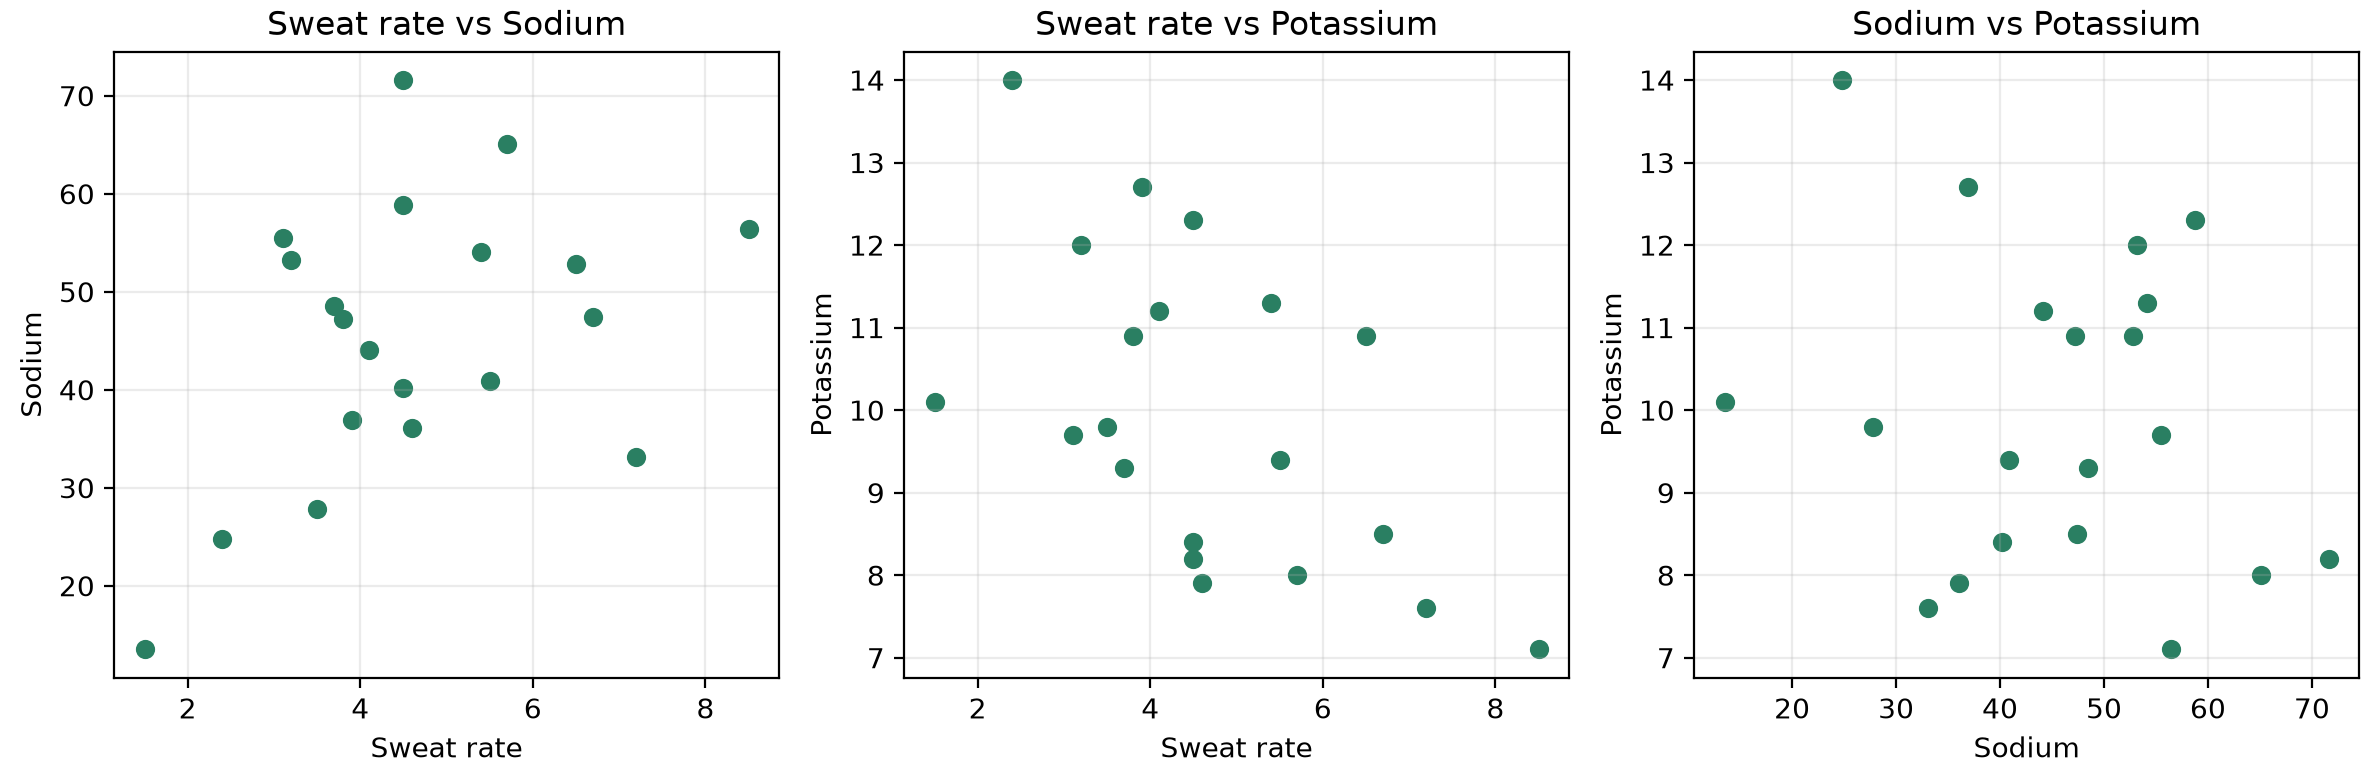
\includegraphics[width=0.96\textwidth,height=0.52\textheight,keepaspectratio]{exercise_5_4_scatter.png}
  \end{center}
  \vspace{-0.15cm}
  \begin{block}{Nhận xét}
    Các scatter plot không cho thấy dạng phi tuyến rõ rệt hay ngoại lệ quá mạnh.
    Kết hợp với Q--Q plot, giả thiết chuẩn đa biến là hợp lý ở mức kiểm tra trực quan.
  \end{block}
\end{frame}

\begin{frame}{Bài tập và ví dụ tính toán}
  \small
  {\large\textbf{Bài 5.5: đề bài trong sách}\par}
  \vspace{0.15cm}
  \begin{block}{Đề bài}
    Các đại lượng \(\bar{\vect{x}}\), \(\mat{S}\) và \(\mat{S}\inv\) được cho trong Ví dụ 5.3 đối với dữ liệu bức xạ lò vi sóng sau khi biến đổi. Hãy kiểm định giả thuyết không
    \[
      H_0:\vect{\mu}\trans=[0{,}55,\ 0{,}60]
    \]
    ở mức ý nghĩa \(\alpha=0{,}05\). Kết quả của bạn có nhất quán với elip tin cậy \(95\%\) cho \(\vect{\mu}\) được vẽ trong Hình 5.1 hay không? Hãy giải thích.
  \end{block}
\end{frame}

\begin{frame}{Bài tập và ví dụ tính toán}
  \small
  {\large\textbf{Bài 5.5: thống kê kiểm định \(T^2\)}\par}
  \vspace{0.1cm}
  \begin{columns}[T,onlytextwidth]
    \column{0.48\textwidth}
    \begin{block}{Dữ liệu từ Ví dụ 5.3}
      \[
        \bar{\vect{x}}=
        \begin{bmatrix}
          0{,}564\\
          0{,}603
        \end{bmatrix},
        \qquad
        \vect{\mu}_0=
        \begin{bmatrix}
          0{,}55\\
          0{,}60
        \end{bmatrix}
      \]
      \[
        \mat{S}\inv=
        \begin{bmatrix}
          203{,}018 & -163{,}391\\
          -163{,}391 & 200{,}228
        \end{bmatrix}.
      \]
    \end{block}

    \column{0.48\textwidth}
    \begin{block}{Tính toán}
      \[
        \vect{d}=\bar{\vect{x}}-\vect{\mu}_0
        =
        \begin{bmatrix}
          0{,}014\\
          0{,}003
        \end{bmatrix}
      \]
      \[
      \begin{aligned}
        T^2
        &=n\vect{d}\trans\mat{S}\inv\vect{d}\\
        &=42[\,0{,}014,\ 0{,}003\,]\mat{S}\inv
          \begin{bmatrix}0{,}014\\0{,}003\end{bmatrix}\\
        &=1{,}170.
      \end{aligned}
      \]
    \end{block}
  \end{columns}
\end{frame}

\begin{frame}{Bài tập và ví dụ tính toán}
  \small
  {\large\textbf{Bài 5.5: minh họa trên Hình 5.1}\par}
  \vspace{0.05cm}
  \begin{columns}[T,onlytextwidth]
    \column{0.58\textwidth}
    \centering
    \begin{tikzpicture}
      \node[anchor=south west,inner sep=0] (fig) at (0,0) {
        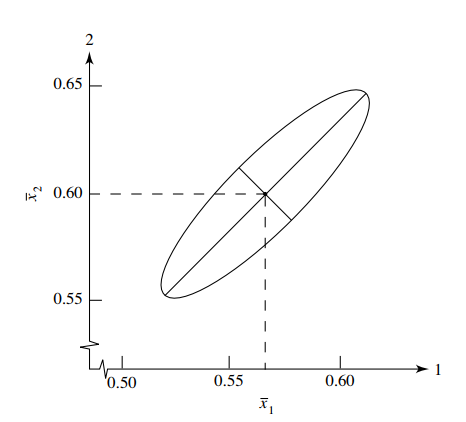
\includegraphics[height=0.64\textheight]{exercise_5_5_fig5_1.png}
      };
      \begin{scope}[x={(fig.south east)},y={(fig.north west)}]
        \filldraw[red!85!black, draw=white, line width=0.7pt] (0.491,0.540) circle (2.5pt);
        \node[red!85!black, font=\scriptsize\bfseries, anchor=south west] at (0.505,0.555) {\(\vect{\mu}_0\)};
      \end{scope}
    \end{tikzpicture}

    \column{0.38\textwidth}
    \begin{block}{Nhận xét}
      \footnotesize
      Điểm đỏ biểu diễn
      \[
        \vect{\mu}_0\trans=[0{,}55,\ 0{,}60].
      \]
      Điểm này nằm trong elip tin cậy \(95\%\), nên kết luận không bác bỏ \(H_0\) là phù hợp với Hình 5.1.
    \end{block}
  \end{columns}
\end{frame}

\begin{frame}{Bài tập và ví dụ tính toán}
  \small
  {\large\textbf{Bài 5.5: quyết định kiểm định}\par}
  \vspace{0.1cm}
  Kiểm định
  \[
    H_0:\vect{\mu}\trans=[0{,}55,\ 0{,}60]
    \qquad\text{với}\qquad
    \alpha=0{,}05.
  \]
  Giá trị tới hạn:
  \[
    \frac{(n-1)p}{n-p}F_{p,n-p}(\alpha)
    =
    \frac{41(2)}{40}F_{2,40}(0{,}05)
    =6{,}625.
  \]

  \begin{alertblock}{Kết luận}
    Vì \(T^2=1{,}170<6{,}625\), ta không bác bỏ \(H_0\).
    Kết quả nhất quán với elip tin cậy \(95\%\) trong Hình 5.1, vì điểm \([0{,}55,\ 0{,}60]\trans\) nằm trong miền tin cậy.
  \end{alertblock}
\end{frame}

% END: Bai 5.4--5.5


\hustcontactpage{Trao đổi}{
  \textbf{Chủ đề:} Suy luận về vectơ trung bình trong phân tích số liệu đa biến\\
  \vspace{0.4cm}
  \textit{Các phần slide được chia theo mục trong thư mục \texttt{sections/}.}
}

\hustthankyou

\end{document}
